% oss-plantilla: oss-2026.10
% Preámbulo corporativo fijo. No editar en sd-NN.tex: exportar_latex.py verificar lo compara byte a byte.
% Para cambiar el formato, editar esta plantilla u oss.sty y subir la versión de la primera línea.
\PassOptionsToPackage{unicode}{hyperref}
\PassOptionsToPackage{hyphens}{url}
\documentclass[11pt]{article}
\usepackage{amsmath,amssymb}
\usepackage{fontspec}
\defaultfontfeatures{Ligatures=TeX,Scale=MatchLowercase}
\setmainfont{DejaVu Sans}
\setsansfont{DejaVu Sans}
\setmonofont{DejaVu Sans Mono}
\usepackage[letterpaper,margin=20mm]{geometry}
\usepackage{microtype}
\usepackage{parskip}
\usepackage{xcolor}
\usepackage{longtable,booktabs,array}
\usepackage{calc}
\usepackage{etoolbox}
\makeatletter
\patchcmd\longtable{\par}{\if@noskipsec\mbox{}\fi\par}{}{}
\makeatother
\usepackage{footnotehyper}
\makesavenoteenv{longtable}
\usepackage{graphicx}
\makeatletter
\newsavebox\pandoc@box
\newcommand*\pandocbounded[1]{%
  \sbox\pandoc@box{#1}%
  \Gscale@div\@tempa{\textheight}{\dimexpr\ht\pandoc@box+\dp\pandoc@box\relax}%
  \Gscale@div\@tempb{\linewidth}{\wd\pandoc@box}%
  \ifdim\@tempb\p@<\@tempa\p@\let\@tempa\@tempb\fi
  \ifdim\@tempa\p@<\p@\scalebox{\@tempa}{\usebox\pandoc@box}%
  \else\usebox{\pandoc@box}%
  \fi}
\def\maxwidth{\ifdim\Gin@nat@width>\linewidth\linewidth\else\Gin@nat@width\fi}
\def\maxheight{\ifdim\Gin@nat@height>\textheight\textheight\else\Gin@nat@height\fi}
\makeatother
\setkeys{Gin}{width=\maxwidth,height=\maxheight,keepaspectratio}
\makeatletter
\def\fps@figure{htbp}
\makeatother
\usepackage[normalem]{ulem}
\providecommand{\st}[1]{\sout{#1}}
\usepackage{fancyvrb}
\setlength{\emergencystretch}{3em}
\providecommand{\tightlist}{%
  \setlength{\itemsep}{0pt}\setlength{\parskip}{0pt}}
\providecommand{\passthrough}[1]{#1}
\setcounter{secnumdepth}{-\maxdimen}
\usepackage[bidi=default]{babel}
\babelprovide[main,import]{spanish}
\let\LanguageShortHands\languageshorthands
\def\languageshorthands#1{}
\usepackage{bookmark}
\usepackage{xurl}
\urlstyle{same}
\hypersetup{pdflang={es-CL},pdfcreator={Only Simple Solutions - exportar_latex.py}}
\usepackage{oss}
\begin{document}

\ossCover{Presentación\\de la empresa}{Subdocumento 1}
\tableofcontents
\clearpage

\hypertarget{capuxedtulo-1-introducciuxf3n}{%
\section{Capítulo 1 · Introducción}\label{capuxedtulo-1-introducciuxf3n}}

Este subdocumento presenta a Only Simple Solutions como proponente: su perfil y capacidades (1.1), organización y dotación (1.2), gobierno interno (1.3), experiencia y certificaciones (1.4), estructura de ejecución para Ancoa (1.5) y alianzas tecnológicas (1.6). El resumen de las experiencias se relaciona con el Formulario T-6, que se prepara y entrega por separado conforme al Comunicado 10. El equipo nominado, sus credenciales y las alianzas específicas del contrato se desarrollan en el Capítulo 12 y en el Formulario T-8.

\hypertarget{presentaciuxf3n-de-la-empresa}{%
\section{1.1 Presentación de la empresa}\label{presentaciuxf3n-de-la-empresa}}

Only Simple Solutions es la empresa proponente de la licitación ficticia TFEP-01/2026. Según el perfil institucional aportado para esta propuesta, fue fundada en Santiago en 2016, mantiene una oficina regional en Concepción y desarrolla software a medida e integra sistemas transaccionales. El perfil declara una dotación de 85 profesionales y una trayectoria de 14 proyectos, seis de ellos vigentes. Estas cifras se presentan como antecedentes de la simulación y deberán conciliarse con la dotación por área, los contratos de referencia y los formularios antes de la entrega.

Su oferta se organiza en cinco líneas de servicio: modernización gradual de sistemas legados; desarrollo de aplicaciones transaccionales a medida; arquitectura e integración de sistemas locales, de nube e híbridos; operación y soporte; y aseguramiento de calidad y pruebas. La empresa reutiliza componentes, patrones y procedimientos de proyectos previos, sin presentar un producto estándar cerrado como solución al caso de Ancoa.

Las capacidades descritas para la compañía son una fábrica de software, una célula de datos, una célula de seguridad de la información y una mesa de servicio. La fábrica se encarga de construir e integrar componentes; la célula de datos aborda integración, calidad y migración; seguridad define y verifica controles; y la mesa de servicio atiende incidentes, problemas y continuidad. La aplicación concreta de estas capacidades al contrato se describe en 1.5. Las experiencias relacionadas con continuidad de puntos de venta, información financiera e integración omnicanal se resumen en 1.4 y deberán individualizarse en el Formulario T-6.

La visión institucional declarada es alcanzar reconocimiento regional en la modernización de sistemas transaccionales hacia 2032. Para este contrato, esa orientación se traduce en preservar la operación de las 22 tiendas y dos centros de distribución mientras se integran las plataformas existentes y se mantiene la separación entre el negocio de retail y el emisor de crédito. La continuidad, la trazabilidad de decisiones y la protección de la información guían el trabajo de los frentes descritos en las secciones siguientes.

\hypertarget{estructura-organizacional}{%
\section{1.2 Estructura Organizacional}\label{estructura-organizacional}}

La estructura corporativa declarada por Only Simple Solutions reúne dirección general y cuatro capacidades operativas: fábrica de software, datos, seguridad de la información y mesa de servicio. Esta relación funcional explica quién proporciona recursos y supervisión a los contratos. El equipo de 16 profesionales previsto para Ancoa es una asignación de proyecto y se presenta por separado en 1.5; no se suma a la dotación corporativa de 85 personas.

\begin{figure}
\centering
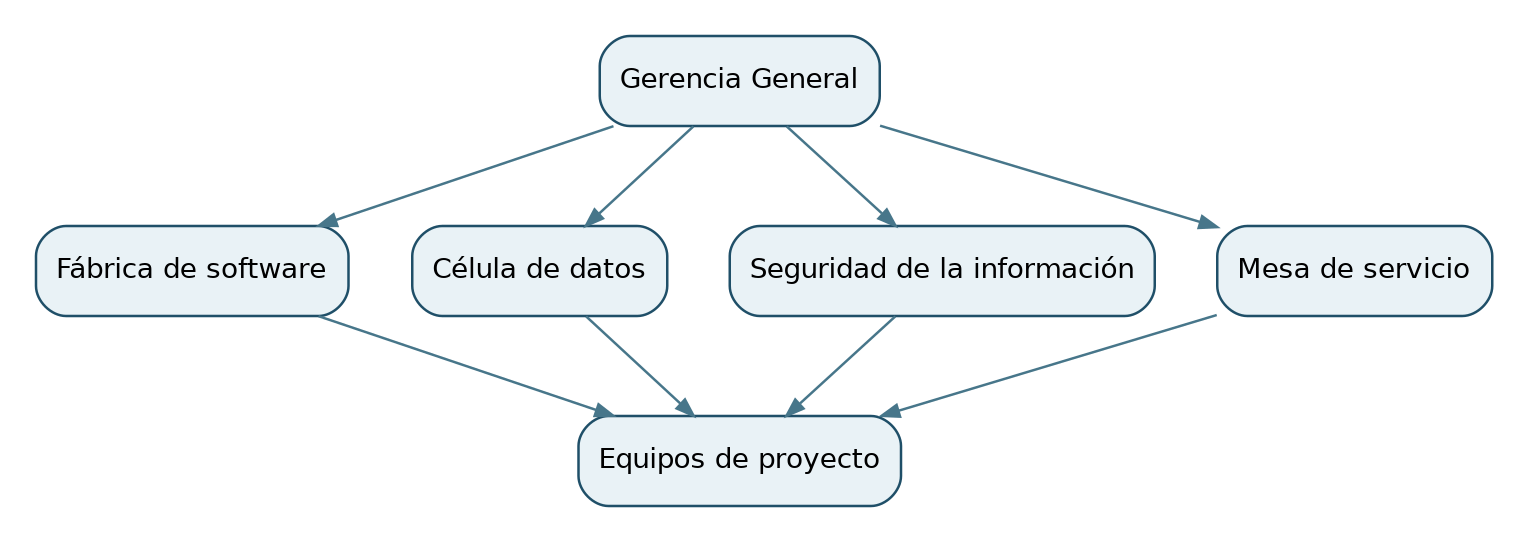
\includegraphics{figuras/diag-01-02_estructura-corporativa-b3efcbcfb9.png}
\caption{Esquema funcional de capacidades corporativas}
\end{figure}

\textbf{Figura 1. Esquema funcional de capacidades corporativas.} Muestra la relación entre dirección, capacidades compartidas y equipos de proyecto; no representa una nómina nominal ni líneas de reporte individual.

\begin{longtable}[]{@{}
  >{\raggedright\arraybackslash}p{(\columnwidth - 4\tabcolsep) * \real{0.3333}}
  >{\raggedright\arraybackslash}p{(\columnwidth - 4\tabcolsep) * \real{0.3333}}
  >{\raggedright\arraybackslash}p{(\columnwidth - 4\tabcolsep) * \real{0.3333}}@{}}
\toprule\noalign{}
\begin{minipage}[b]{\linewidth}\raggedright
Capacidad permanente
\end{minipage} & \begin{minipage}[b]{\linewidth}\raggedright
Función en la oferta
\end{minipage} & \begin{minipage}[b]{\linewidth}\raggedright
Dotación corporativa por área
\end{minipage} \\
\midrule\noalign{}
\endhead
\bottomrule\noalign{}
\endlastfoot
Fábrica de software & Arquitectura, desarrollo e integración & Por conciliar con nómina institucional \\
Célula de datos & Gobierno, calidad, integración y migración & Por conciliar con nómina institucional \\
Seguridad de la información & Riesgos, controles y respuesta a incidentes & Por conciliar con nómina institucional \\
Mesa de servicio & Monitoreo, soporte y conocimiento operativo & Por conciliar con nómina institucional \\
\end{longtable}

La distribución de los 85 profesionales entre estas capacidades aún requiere respaldo. La matriz de dedicación y el equipo nominado del contrato se desarrollan en el Capítulo 12 y en el Formulario T-8, conforme al índice obligatorio del Comunicado 10.

\hypertarget{gobierno-interno-calidad-seguridad-y-conocimiento}{%
\section{1.3 Gobierno interno Calidad, Seguridad y Conocimiento}\label{gobierno-interno-calidad-seguridad-y-conocimiento}}

El modelo de gobierno declarado para Only Simple Solutions comprende políticas, responsables e instancias de seguimiento. Las prácticas descritas a continuación se alinean con normas de gestión; la acreditación de una certificación institucional requiere un certificado independiente con emisor, alcance y vigencia, según 1.4.

\hypertarget{calidad}{%
\subsection{1.3.1 Calidad}\label{calidad}}

La Gerencia General es responsable de aprobar la política de calidad. El Líder de Calidad coordina su aplicación y mantiene independencia funcional frente a quienes construyen los componentes evaluados. El modelo descrito contempla revisión anual por la dirección, comité trimestral de mejora, auditorías internas anuales y seguimiento de no conformidades del proyecto semanal durante construcción y mensual durante operación.

La evidencia necesaria para demostrar su ejecución comprende política aprobada y versionada, actas de comité y revisión, programa e informes de auditoría, registro de no conformidades con responsables y cierre, y trazabilidad entre requisitos, pruebas y aceptación. El texto del proyecto sigue un enfoque alineado con ISO 9001; la eventual certificación se declara y acredita por separado.

\hypertarget{seguridad-de-la-informaciuxf3n}{%
\subsection{1.3.2 Seguridad de la información}\label{seguridad-de-la-informaciuxf3n}}

El Encargado de Seguridad de la Información coordina la clasificación de la información, el registro de riesgos, las revisiones de acceso y la respuesta a incidentes. El modelo prevé clasificación pública, interna, confidencial y restringida; la información financiera y de tarjetas recibe el nivel restringido y controles de acceso acordes. El comité de seguridad revisa mensualmente riesgos, hallazgos e incidentes; los accesos se revisan trimestralmente y al cambiar los integrantes del proyecto.

Las actas de comité, la matriz de clasificación, los registros de riesgos y accesos, las decisiones de tratamiento y los informes de incidentes son las evidencias previstas. Los controles se diseñan con referencia a ISO/IEC 27001 y 27002, y se consideran las guías 27017 y 27018 para servicios de nube. PCI DSS se trata como estándar aplicable cuando corresponda al tratamiento de datos de tarjetas; su mención no implica certificación institucional obtenida.

\hypertarget{gestiuxf3n-del-conocimiento}{%
\subsection{1.3.3 Gestión del conocimiento}\label{gestiuxf3n-del-conocimiento}}

El Jefe de Proyecto responde por la continuidad del conocimiento dentro del contrato y cada líder de frente por la documentación de su ámbito. Las decisiones técnicas se registrarán con alternativas y fundamento. Manuales, guías de resolución, procedimientos de conmutación y libros de operación llevarán versión, fecha y responsable. La mesa de servicio mantendrá una base de conocimiento alimentada por incidentes y problemas resueltos.

Al cierre de cada hito se revisarán los documentos y se efectuará una transferencia al equipo correspondiente de Ancoa. La evidencia prevista comprende registros de decisión, historial de versiones, artículos de conocimiento, actas de traspaso y constancias de capacitación. Las políticas, actas y registros institucionales anteriores al contrato deberán incorporarse como soporte para acreditar que el gobierno descrito ya opera en la compañía.

\hypertarget{experiencia-y-certificaciones}{%
\section{1.4 Experiencia y Certificaciones}\label{experiencia-y-certificaciones}}

El anexo de trabajo «Informes(8).md», apartado A.2, describe tres experiencias pertinentes al caso: modernización de puntos de venta con operación sin enlace, consentimiento seguro para un emisor financiero e integración de disponibilidad para venta omnicanal y marketplace. En conjunto abordan continuidad comercial, tratamiento de información sensible e integración entre canales. Son antecedentes declarados por el equipo para esta simulación; la verificación de contratos, métricas y contrapartes debe constar en el Formulario T-6 y sus soportes. La mención del anexo permite rastrear el origen de los datos, pero no los valida por sí sola.

\begin{longtable}[]{@{}
  >{\raggedright\arraybackslash}p{(\columnwidth - 4\tabcolsep) * \real{0.3333}}
  >{\raggedright\arraybackslash}p{(\columnwidth - 4\tabcolsep) * \real{0.3333}}
  >{\raggedright\arraybackslash}p{(\columnwidth - 4\tabcolsep) * \real{0.3333}}@{}}
\toprule\noalign{}
\begin{minipage}[b]{\linewidth}\raggedright
Experiencia descrita
\end{minipage} & \begin{minipage}[b]{\linewidth}\raggedright
Pertinencia para Ancoa
\end{minipage} & \begin{minipage}[b]{\linewidth}\raggedright
Acreditación pendiente en T-6
\end{minipage} \\
\midrule\noalign{}
\endhead
\bottomrule\noalign{}
\endlastfoot
Modernización de puntos de venta y continuidad sin enlace (2022--2023) & Venta local y sincronización tras recuperar conectividad; el anexo declara arquitectura híbrida, 25 sucursales y continuidad local mínima de 12 horas & Rango de monto, SLA de 99,5 \% y volumen de 500.000 transacciones/mes marcados como estimados; faltan resultado de SLA, contrato y contacto nominal \\
Consentimiento seguro para emisor financiero (2024) & Evidencia de consentimiento y trazabilidad para una cartera declarada de 450.000 deudores & Rango de monto, SLA de 99,9 \% y volumen de 1.000.000 de operaciones/mes marcados como estimados; faltan resultado de SLA, contrato y contacto nominal \\
Motor de disponibilidad e integración de marketplace (2023--2024) & Inventario comprometible y coordinación de pedidos entre canales; se declaran 30 tiendas y 200 vendedores externos & El anexo atribuye el proyecto a una empresa real ajena a la simulación; debe corregirse el mandante. Monto, arquitectura, SLA y 150 transacciones/segundo están marcados como estimados; faltan resultado de SLA, contrato y contacto nominal \\
\end{longtable}

El anexo \textbf{identifica} los proyectos primero y tercero como híbridos y declara SLA comprometidos de 99,5 \% o más en los tres. Hasta completar el T-6 y los soportes no queda \textbf{acreditado} el cumplimiento de esos habilitantes del artículo 34 de las Bases Administrativas. Tampoco se traslada la autonomía de 12 horas declarada para el proyecto anterior como compromiso para Ancoa: este último necesita una cifra única, dimensionada y coherente entre arquitectura, operación y pruebas. Las mejoras de negocio que enumera el anexo ---por ejemplo, ventas preservadas, reducción de reclamos y cancelaciones--- requieren línea base, período, fuente de medición y validación de la contraparte antes de citarlas como resultados comprobados.

\hypertarget{certificaciones-institucionales}{%
\subsection{1.4.1 Certificaciones institucionales}\label{certificaciones-institucionales}}

Las prácticas de calidad, seguridad, privacidad y continuidad descritas en 1.3 toman como referencia ISO 9001, ISO/IEC 27001, ISO/IEC 27701 e ISO 22301. El borrador recibido las presentaba como certificaciones obtenidas, pero no incluía certificado, emisor, código, alcance ni fecha de vigencia. Por ello, su acreditación queda pendiente y no se declaran aquí como certificados vigentes.

\begin{longtable}[]{@{}
  >{\raggedright\arraybackslash}p{(\columnwidth - 4\tabcolsep) * \real{0.3333}}
  >{\raggedright\arraybackslash}p{(\columnwidth - 4\tabcolsep) * \real{0.3333}}
  >{\raggedright\arraybackslash}p{(\columnwidth - 4\tabcolsep) * \real{0.3333}}@{}}
\toprule\noalign{}
\begin{minipage}[b]{\linewidth}\raggedright
Norma
\end{minipage} & \begin{minipage}[b]{\linewidth}\raggedright
Estado documental para esta propuesta
\end{minipage} & \begin{minipage}[b]{\linewidth}\raggedright
Soporte necesario
\end{minipage} \\
\midrule\noalign{}
\endhead
\bottomrule\noalign{}
\endlastfoot
ISO/IEC 27001 & Pendiente de acreditar & Certificado vigente; si no existe, plan formal firmado con hitos verificables dentro de los primeros doce meses, según artículo 34 \\
ISO 9001 & Pendiente de acreditar & Certificado, alcance y vigencia si se declara como certificación institucional \\
ISO/IEC 27701 e ISO 22301 & Pendientes de acreditar & Certificado y vigencia si se mantienen como certificaciones declaradas \\
PCI DSS & Estándar de control mencionado en 1.3 & Evaluación de aplicabilidad y evidencia del alcance; no se presenta como certificación obtenida \\
\end{longtable}

La capacidad descrita puede respaldar el contrato de Ancoa una vez que los tres proyectos, las credenciales y sus evidencias sean consistentes entre este resumen, el T-6, el T-8 y los soportes institucionales. Las referencias normativas y documentales usadas para esta sección se registran en el maestro del subdocumento.

\hypertarget{estructura-para-proyecto}{%
\section{1.5 Estructura para Proyecto}\label{estructura-para-proyecto}}

Only Simple Solutions organizará el contrato de 56 meses bajo un Jefe de Proyecto y frentes de arquitectura y desarrollo, seguridad, datos, calidad, operación e implantación. El equipo funcional descrito en el borrador suma 16 profesionales. Su asignación y dedicación por período deberán conciliarse con el Capítulo 12, el Formulario T-8 y la nivelación de recursos; la cifra de 16 no equivale a presencia de jornada completa de todos los perfiles durante los 56 meses.

\begin{longtable}[]{@{}
  >{\raggedright\arraybackslash}p{(\columnwidth - 6\tabcolsep) * \real{0.2500}}
  >{\raggedright\arraybackslash}p{(\columnwidth - 6\tabcolsep) * \real{0.2500}}
  >{\raggedleft\arraybackslash}p{(\columnwidth - 6\tabcolsep) * \real{0.2500}}
  >{\raggedright\arraybackslash}p{(\columnwidth - 6\tabcolsep) * \real{0.2500}}@{}}
\toprule\noalign{}
\begin{minipage}[b]{\linewidth}\raggedright
Frente
\end{minipage} & \begin{minipage}[b]{\linewidth}\raggedright
Roles previstos
\end{minipage} & \begin{minipage}[b]{\linewidth}\raggedleft
Personas
\end{minipage} & \begin{minipage}[b]{\linewidth}\raggedright
Aplicación al caso
\end{minipage} \\
\midrule\noalign{}
\endhead
\bottomrule\noalign{}
\endlastfoot
Dirección & Jefe de Proyecto & 1 & Plazos, riesgos, cambios y relación contractual \\
Arquitectura y construcción & Arquitecto de Solución; ingenieros de solución y desarrollo & 3 & Arquitectura híbrida, levantamiento de nueve plataformas y catorce interfaces, integración y construcción \\
Seguridad & Encargado y analista de seguridad & 2 & Separación entre retail y crédito, accesos, riesgos y respuesta a incidentes \\
Datos & Líder e ingenieros de datos & 3 & Calidad, migración y conciliación de información, incluida la cartera de crédito \\
Calidad & Líder e ingenieros QA & 3 & Trazabilidad de requisitos, pruebas y evidencias de aceptación \\
Operación & Líder de Operación e ingeniero DevOps y soporte & 2 & Monitoreo, continuidad, recuperación y soporte \\
Implantación & Líder de Implantación y especialista de capacitación & 2 & Marchas blancas, despliegue en tiendas y capacitación por perfil y turno \\
\textbf{Total} & & \textbf{16} & \\
\end{longtable}

\begin{figure}
\centering
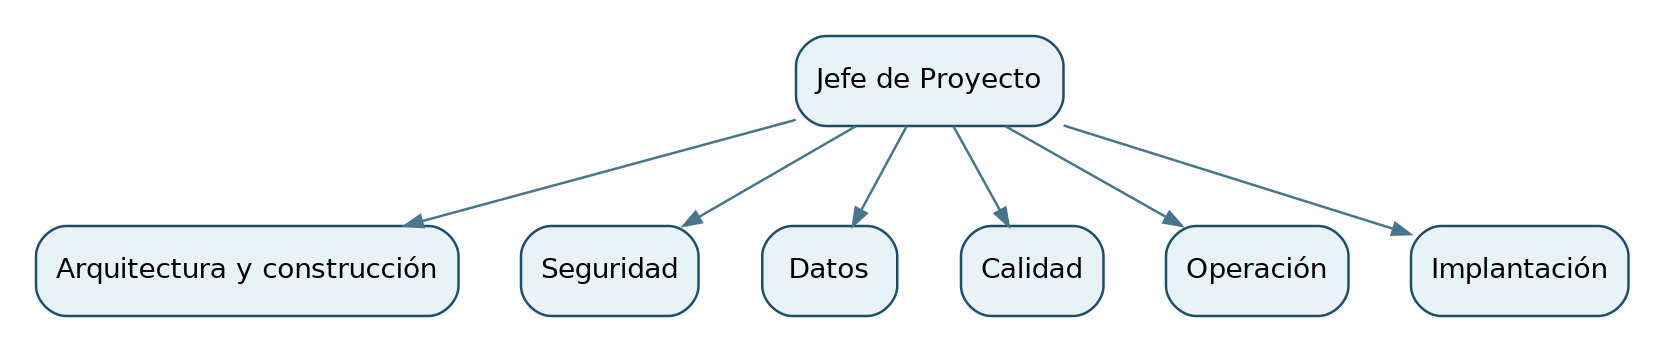
\includegraphics{figuras/diag-01-05_estructura-proyecto-1d677ea629.png}
\caption{Frentes del proyecto}
\end{figure}

\textbf{Figura 2. Frentes del proyecto.} Cada líder informa a la jefatura del contrato; Calidad mantiene independencia funcional para registrar desviaciones y objetar liberaciones.

La jefatura coordinará a la Contraparte Técnica de Ancoa mediante seguimiento semanal y un Comité de Proyecto quincenal. Los asuntos estratégicos y los cambios de alcance se elevarán al Comité Ejecutivo mensual. Las decisiones técnicas se revisarán en el Comité de Arquitectura mensual. Desde la preparación operativa se revisarán incidentes, niveles de servicio y transferencia; la operación contractual de 36 meses corresponde a los meses 21 a 56.

La cobertura específica de arquitectura de nube, integración, administración de bases de datos, mesa de servicio y soporte en terreno debe asignarse por nombre o función dentro de los frentes y reflejarse en la matriz de dedicación por meses. Las fichas curriculares, certificaciones individuales y cartas de compromiso del equipo nominado pertenecen al Capítulo 12 y al T-8. Su acreditación queda pendiente del anexo del equipo.

\hypertarget{alianzas}{%
\section{1.6 Alianzas}\label{alianzas}}

El borrador identifica tecnologías de Microsoft Azure, Fortinet y Dell Technologies como posibles apoyos de nube, seguridad de redes e infraestructura local. Esa identificación describe componentes y fabricantes considerados; la condición de socio comercial de Only Simple Solutions o de un integrador participante requiere un certificado o acuerdo vigente.

\begin{longtable}[]{@{}
  >{\raggedright\arraybackslash}p{(\columnwidth - 4\tabcolsep) * \real{0.3333}}
  >{\raggedright\arraybackslash}p{(\columnwidth - 4\tabcolsep) * \real{0.3333}}
  >{\raggedright\arraybackslash}p{(\columnwidth - 4\tabcolsep) * \real{0.3333}}@{}}
\toprule\noalign{}
\begin{minipage}[b]{\linewidth}\raggedright
Ámbito
\end{minipage} & \begin{minipage}[b]{\linewidth}\raggedright
Proveedor mencionado en el borrador
\end{minipage} & \begin{minipage}[b]{\linewidth}\raggedright
Evidencia pendiente
\end{minipage} \\
\midrule\noalign{}
\endhead
\bottomrule\noalign{}
\endlastfoot
Nube pública & Microsoft Azure & Nivel de socio, identificador, alcance, vigencia y certificado del proveedor o carta de compromiso de un socio certificado que participe en el proyecto \\
Seguridad de redes & Fortinet & Contrato o carta vigente que precise entidad aliada, servicios y responsabilidad \\
Infraestructura local & Dell Technologies o integrador & Contrato o carta vigente que precise proveedor, servicios y responsabilidad \\
\end{longtable}

El artículo 34 de las Bases exige acreditar la condición de socio del proveedor de nube ofertado o un acuerdo formal con un socio certificado que participe en el proyecto. Hasta contar con ese soporte, la relación comercial no se presenta como alianza vigente demostrada. El proveedor finalmente declarado aquí deberá coincidir con la arquitectura física, el Capítulo 12 y la matriz de cumplimiento técnico. Las alianzas específicas para la ejecución de Ancoa se desarrollan en 12.3.

\ossFinalPage

\end{document}
